\documentclass{bioinfo}
\copyrightyear{2016} \pubyear{2016}

%% Some pieces required from the pandoc template
\providecommand{\tightlist}{%
  \setlength{\itemsep}{0pt}\setlength{\parskip}{0pt}}


% Pandoc citation processing


% hyperref makes the margins screwy.
% https://groups.google.com/forum/#!topic/latexusersgroup/4W_SwGk6zx4
% http://ansuz.sooke.bc.ca/software/latex-tricks.php
% \usepackage[colorlinks=true, allcolors=blue]{hyperref}

\access{Advance Access Publication Date:   }
\appnotes{Manuscript Category}

\begin{document}
\firstpage{1}

\subtitle{Application Note}

\title[JBrowseR: R Interface to JBrowse 2]{JBrowseR: An R Interface to
the JBrowse 2 Genome Browser}

\author[FirstAuthorLastName \textit{et~al}.]{
Elliot Hershberg\,\textsuperscript{1},
Garrett Stevens\,\textsuperscript{1},
Colin Diesh\,\textsuperscript{1},
Peter Xie\,\textsuperscript{1},
Teresa De Jesus Martinez\,\textsuperscript{1},
Rob Buels\,\textsuperscript{1},
Lincoln Stein\,\textsuperscript{2},
Ian Holmes\,\textsuperscript{1*},
}

\address{
\textsuperscript{1}Department of Bioengineering, University of
California, Berkeley, Berkeley, CA 94720, USA\\
\textsuperscript{2}Ontario Institute for Cancer Research, Toronto, ON
M5G 0A3, Canada\\
}

\corresp{*To whom correspondence should be addressed. E-mail:
ihh@berkeley.edu}

\history{Received on XXX; revised on XXX; accepted on XXX}

\editor{Associate Editor: XXX}

\abstract{
\textbf{Motivation:} Genome browsers are an essential tool in genome
analysis. Modern genome browsers enable complex and interactive
visualization of a wide variety of genomic data modalities. While such
browsers are very powerful, they can be challenging to configure and
program for bioinformaticians lacking expertise in web development.\\
\textbf{Results:} We have developed an R package that provides an
interface to the JBrowse 2 genome browser. The package can be used to
configure and customize the browser entirely with R code. The browser
can be deployed from the R console, or embedded in Shiny applications or
R Markdown documents.\\
\textbf{Availability:} JBrowseR is available for download from CRAN, and
the source code is openly available from the Github repository at\\
\textbf{Contact:}ihh@berkeley.edu\\
\textbf{Supplementary information:} Supplementary data are available at
Bioinformatics Online.}

\maketitle

\section{Introduction}

The development of genome browsers is widely considered to be one of the
fundamental milestones of the genomic revolution
\citep{packer2007clickable}. Genome browsers provide researchers the
ability to visually display and explore genomic annotations and data.
Due to their widespread adoption and use, the linear display of genomic
information along reference coordinates is one of the most common
represenations of biological data in the 21st century.

Since their original development during the advent of genome sequencing
\citep{kent2002human, birney2004overview}, genome browsers have made
considerable gains in performance and sophistication. One important
development has been the implementation of genome browsers in
JavaScript, beginning with JBrowse \citep{buels2016jbrowse}. Leveraging
JavaScript makes it possible to move computation that previously took
place on a server into the client browser. Another core advantage of
JavaScript based browsers is that they can leverage modern web
technologies such as Canvas and SVG, providing a more responsive and
interactive experience for the user.

More recently, JBrowse has been rewritten using newer web technologies
such as ReactJS and TypeScript to create an extensible platform for
visualizing and integrating biological data called JBrowse 2. The
platform can be configured and deployed with custom data and settings.
This architecture enables research communities to develop and maintain
curated sets of resources and data on the web, such as WormBase for the
\emph{C. elegans} community \citep{harris2010wormbase}. A new product
offering of JBrowse 2 is a React component that renders a configurable
genome browser, enabling researchers to embed custom browsers into
existing React applications.

While the JBrowse 2 React component is powerful and extensible, it can
present a steep learning curve for bioinformaticians who don't have
experience with React development. On the other hand, the R programming
language and environment is widely used in the bioinformatics community,
as evidenced by the size and and usage of efforts such as Bioconductor
\citep{huber2015orchestrating}. To bridge this gap, we introduce
JBrowseR, an R interface the JBrowse 2 genome browser. JBrowseR is an R
package with functions for embedding a custom browser instance in a
Shiny app, R Markdown document, or the R console.

\section{Materials and Methods}

JBrowseR is implemented as an R package and distributed on CRAN. The
package was built according to R best practices, leveraging the devtools
package. The core rendering methods of the library rely on the
htmlwidgets framework, which can be used to embed JavaScript
visualization tools in R Shiny apps, as well as R Markdown documents.
Htmlwidgets can also can be used from an R interactive console. Using
the reactR package, JBrowseR renders the JBrowse 2 widget inside of a
root HTML element in an htmlwidget.

The interface of JBrowseR enables users to generate JBrowse 2
configuration for their own data using simple R functions. The
configuration values can be composed together to create an arbitrarily
complex custom browser. The majority of major genomic data types
displayed in genome browsers are supported. JBrowseR also includes a
HTTP server for serving local data that is configured with the necessary
settings and features for working with genome browsers such as JBrowse
and IGV.js \citep{robinson2011integrative, robinson2017variant}.

The source code for JBrowseR is hosted on GitHub, and is automatically
tested using continuous integration running on the Windows, MacOS and
Linux operating systems. Automated tests for the package are implemented
using the testthat R package.

\begin{figure}
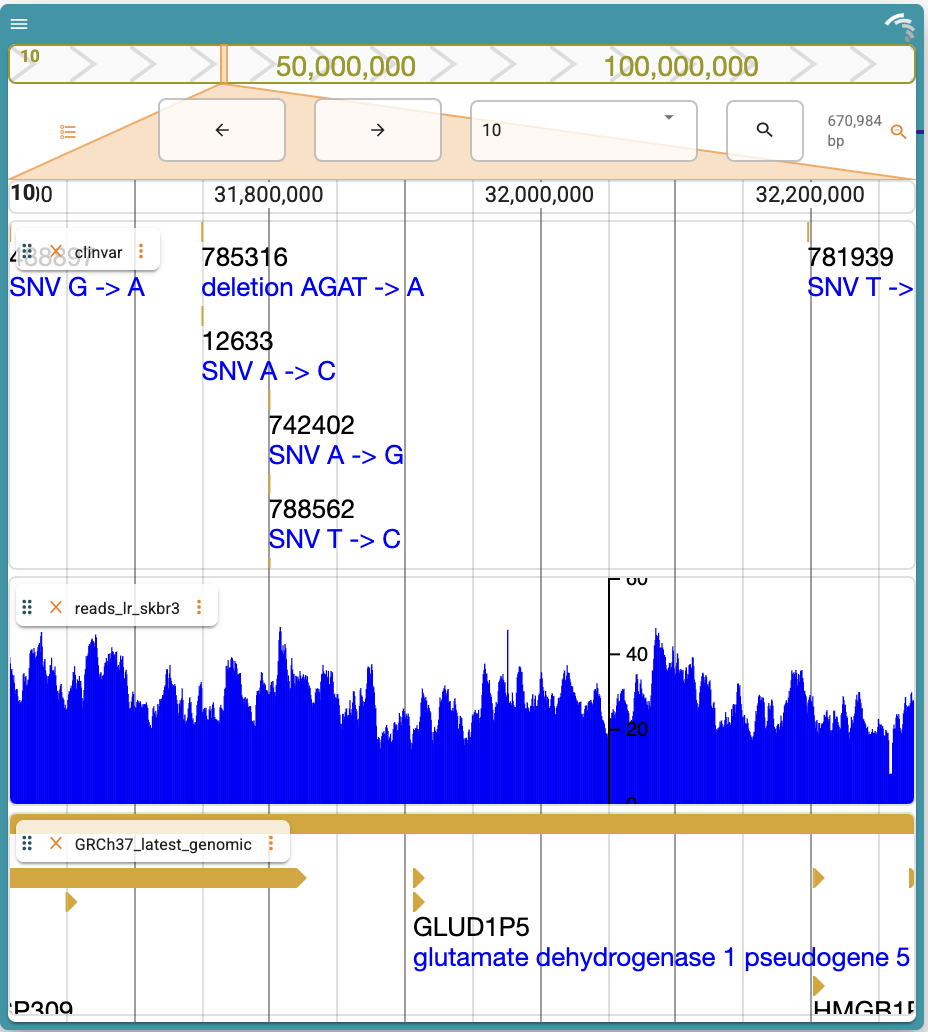
\includegraphics[width=1\linewidth]{JBrowseR-paper-fig1} \caption{A custom JBrowse 2 genome browser generated using JBrowseR.}\label{fig:unnamed-chunk-1}
\end{figure}

\section{Results and discussion}

In order to demonstrate the utility of JBrowseR, several Shiny apps were
built and included along with the package source code on GitHub. One of
the included apps demonstrates adding CRAM, VCF, GFF3, and bigWig data
(fig.~1), as well as setting a custom color palette for the browser.
Another one of the provided demo apps illustrates how JBrowseR can also
be configured with a JSON file like the other JBrowse 2 products by
loading the Sars-CoV-2 reference genome and NCBI annotations from a
JBrowse 2 configuration file. Finally, we have provided an example
deployment of JBrowseR in an app with interactions connected to other R
shiny UI components at
\href{https://elliothershberg.shinyapps.io/sars-cov-2-spike-mutations/}{https://elliothershberg.shinyapps.io/sars-cov-2-spike-mutations/}.

One of the core strengths of JBrowseR is its versatility. It
considerably lowers the level of web development expertise required to
create a genomics application with a fast and flexible genome browser.
However, applications are not the only available target point for the
rendering functions. JBrowseR can embed a genome browser into R
Markdown, which is a flexible documentation format that is widely used
to write scientific articles. We anticipate that as platforms such as
eLife's ``reproducible article'' \citep{maciocci2019introducing} mature
and become more widely adopted, it will be possible for genomics
articles to contain interactive genome browsers such as JBrowseR
displaying their data.

\section{Availability}

The JBrowseR is freely available for download from CRAN, and the source
code is publicly available at
\href{https://github.com/elliothershberg/JBrowseR/}{https://github.com/elliothershberg/JBrowseR/}.
The package reference guide and tutorials can be found at
\href{https://elliothershberg.github.io/JBrowseR/}{https://elliothershberg.github.io/JBrowseR/}.

\section*{Acknowledgements}
\addcontentsline{toc}{section}{Acknowledgements}

???

\section*{Funding}
\addcontentsline{toc}{section}{Funding}

???


% Bibliography
\bibliographystyle{natbib}
\bibliography{bibliography.bib}

\end{document}
